\documentclass[10pt,twocolumn,letterpaper]{article}
\usepackage[UTF8]{ctex}%兼容中文
\usepackage{booktabs}
\usepackage{cite}
\usepackage{cvpr}
\usepackage{times}
\usepackage{epsfig}
\usepackage{graphicx}
\usepackage{amsmath}
\usepackage{amssymb}
\usepackage{comment}
\usepackage{dirtree}

\usepackage{algorithm}  
\usepackage{algpseudocode}  
\usepackage{amsmath}  
\renewcommand{\algorithmicrequire}{\textbf{Input:}}  % Use Input in the format of Algorithm  
\renewcommand{\algorithmicensure}{\textbf{Output:}} % Use Output in the format of Algorithm  



%!BIB program = bibtex
% Include other packages here, before hyperref.

% If you comment hyperref and then uncomment it, you should delete
% egpaper.aux before re-running latex.  (Or just hit 'q' on the first latex
% run, let it finish, and you should be clear).
\usepackage[breaklinks=true,bookmarks=false]{hyperref}
\usepackage[toc,page]{appendix}
\cvprfinalcopy % *** Uncomment this line for the final submission

\def\cvprPaperID{****} % *** Enter the CVPR Paper ID here
\def\httilde{\mbox{\tt\raisebox{-.5ex}{\symbol{126}}}}

% Pages are numbered in submission mode, and unnumbered in camera-ready
%\ifcvprfinal\pagestyle{empty}\fi
\setcounter{page}{1}
\begin{document}

%%%%%%%%% TITLE
\title{Schlieren}

\author{None\\
None\\
None\\
{\tt\small None@none.com}
}
% For a paper whose authors are all at the same institution,
% omit the following lines up until the closing ``}''.
% Additional authors and addresses can be added with ``\and'',
% just like the second author.


\maketitle



\section{引言}

纹影图实验中, 可以通过采集的图像灰度反映对应区域的流场密度.对灰度图进行色彩映射渲染, 能够更好体现出流场密度的变化情况(见图.\ref{fig:first_show}).
\begin{figure}[t]
	\begin{center}
		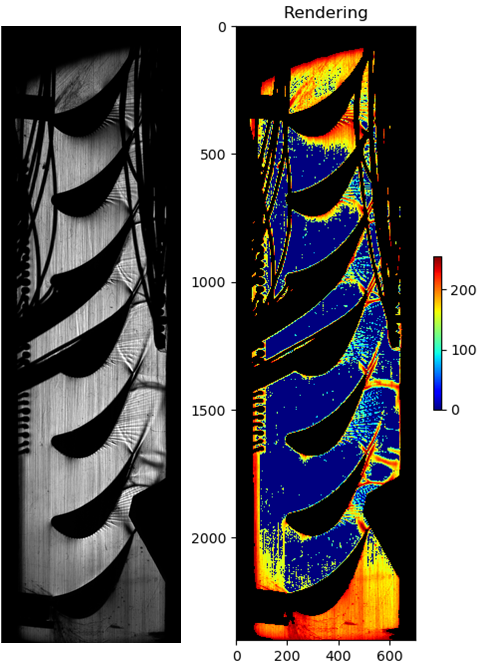
\includegraphics[width=0.75\linewidth]{src/first_show}
	\end{center}
	\caption{ \textbf{Schlieren图结果.}}
	\label{fig:first_show}	
\end{figure}
由于图像的管壁区域中存在线缆, 试件等物体, 对全图直接进行色彩映射, 会被此类区域影响; 另外, 透明管壁上由于气体流动所形成的条纹状划痕, 在图像中会呈现黑色线条噪声, 也会影响映射结果.
所以, 对流场区域分割出来,并单独进行色彩映射, 是解决问题的关键.

\paragraph{问题描述}
根据待处理的纹影图(灰度图), 我们可以将整个区域的像素分为三个像素点集: 定义Rigid为包括管壁, 试件, 线缆等区域, 记做$V_{r}$; 定义Bgk为带有大量纵向条纹噪声的透明管壁区域, 记做$V_{b}$; 定义Flow为流场区域, 记做$V_{f}$.可知

\begin{eqnarray}
	\quad &V= V_{f} \bigcup V_{r} \bigcup V_{b}\\
	\nonumber
	\quad&\forall V_i, V_j, ~~ V_i\bigcap V_j = \oslash,~~ i,j \in \{\text{r,f,b}\}&
	\label{eq:v}
\end{eqnarray}
若有掩膜(Mask)二值函数

\begin{eqnarray}
	M_{f}(p) = \left\{
		\begin{aligned}
			\quad&=&1, ~ p\in V_{f}\\
			\nonumber
			\quad&=&0, ~p \in V - V_{f}
		\end{aligned}
	\right.
	\label{eq:Mf}
\end{eqnarray}


\begin{eqnarray}
	M_{r}(p) = \left\{
		\begin{aligned}
			\quad&=&1, ~ p\in V_{r}\\
			\nonumber
			\quad&=&0, ~p \in V - V_{r}
		\end{aligned}
	\right.
	\label{eq:Mr}
\end{eqnarray}
以及

\begin{eqnarray}
	M_{b}(p) = \left\{
		\begin{aligned}
			\quad&=&1, ~ p\in V_{b}\\
			\nonumber
			\quad&=&0, ~p \in V - V_{b}
		\end{aligned}
	\right.
	\label{eq:Mb}
\end{eqnarray}



则可单独提取出各自区域像素值,如:
\begin{eqnarray}
	\nonumber
	\quad \mathop{I}\limits_{p \in V_{f}}(p)= I(p) M_{f}(p)\\
	\nonumber
	\quad \mathop{I}\limits_{p \in V_{r}}(p)= I(p) M_{r}(p)\\
	\nonumber
	\quad \mathop{I}\limits_{p \in V_{b}}(p)= I(p) M_{b}(p)
\end{eqnarray}
综上, 我们只需要对全图中各个像素进行正确分类, 则可通过分割对流场区域进行提取, 从而实现单独色彩映射.



\begin{figure}[t]
	\begin{center}
		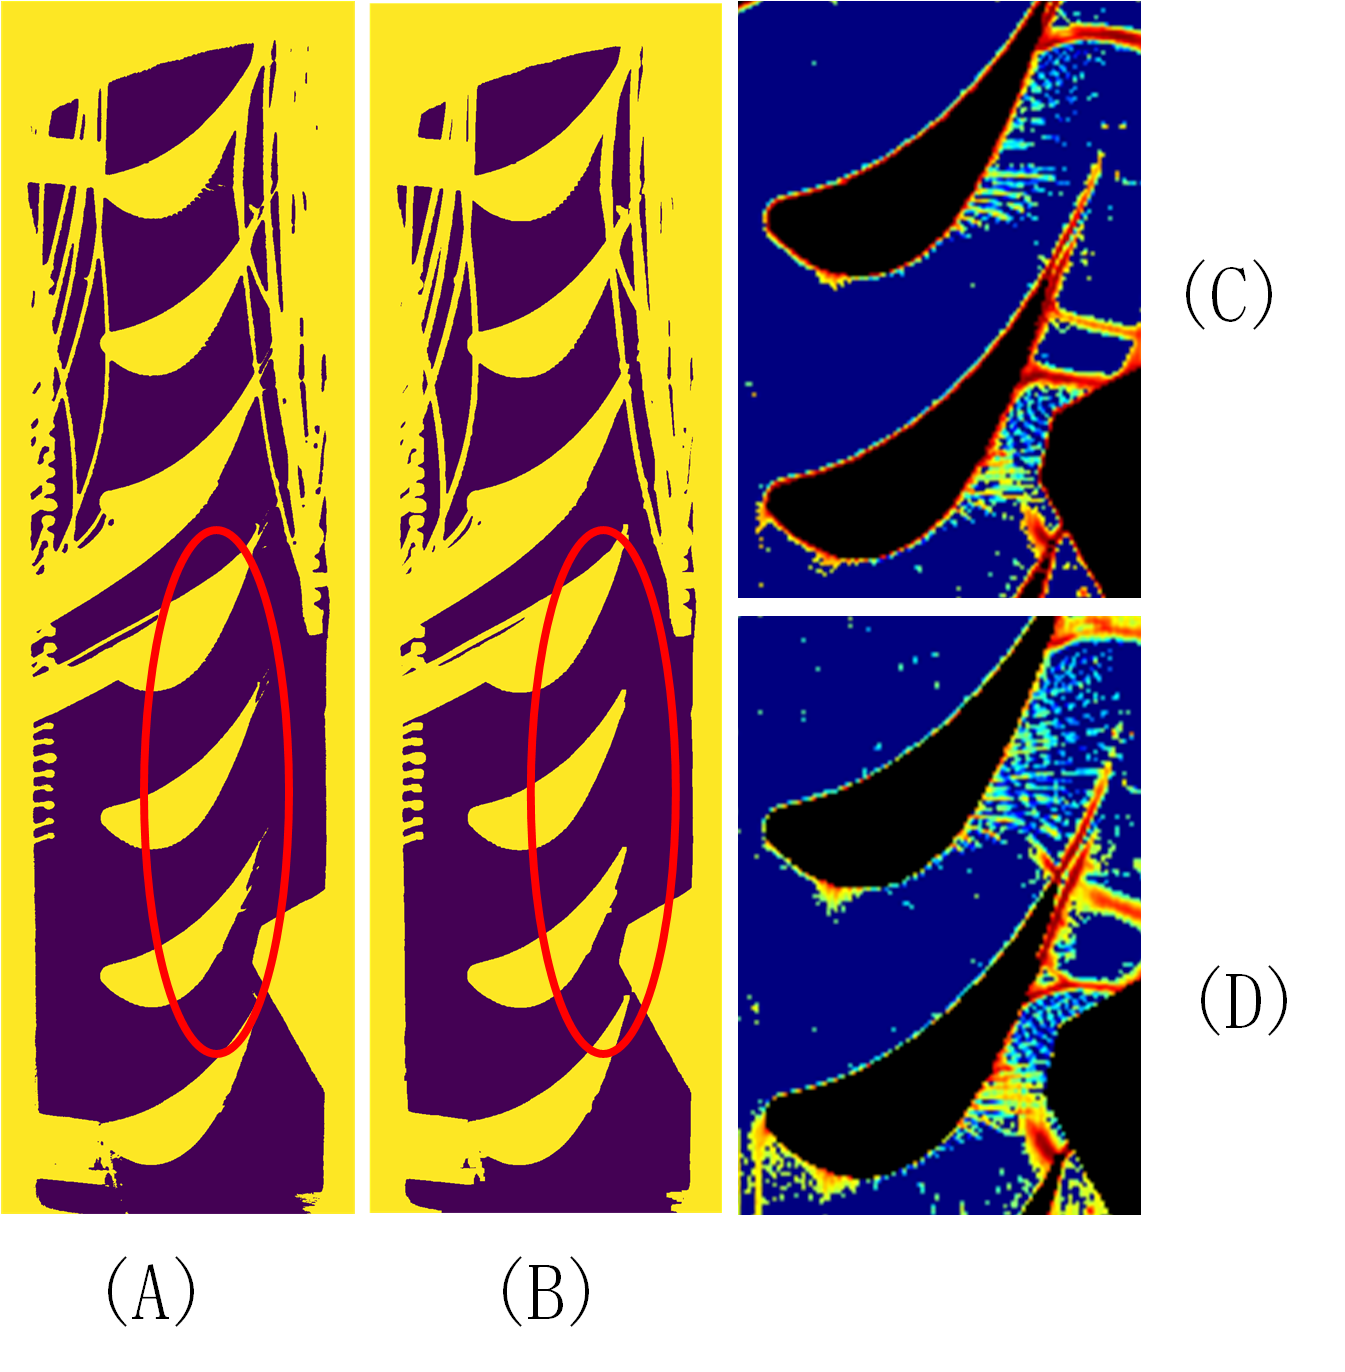
\includegraphics[width=0.75\linewidth]{src/rigid}
	\end{center}
	\caption{(A)(B)分别为$M_r$膨胀腐蚀操作前与操作后,(C)(D)分别为经过处理前与处理后的不同结果. 可以看到膨胀腐蚀操作去除了孤立点(红色圈出), 并且能有效改善叶片边缘处像素分类为Flow区域并带入渲染造成的红圈错误.}
	\label{fig:rigid}	
\end{figure}

\section{Flow区域处理}

Flow区域典型特征就是包含多种方向纹理低灰度条纹, 这使得直接通过门限值过滤方法并不现实. 我们注意到, 在数据中要保留的流场区域的纹理几乎不存在垂直方向, 单背景区域则有大量纵向纹理条纹, 所以我们提出通过纵向纹理抑制,非纵向条纹加深和灰度门限值方法对$V_b$像素进行判别.

具体来说,我们可以通过左右方向的锐化使得非纵向条纹灰度值降低(变黑),纵向条纹灰度模糊(变高),这可通过原图和方向锐化卷积核的卷积实现. 操作后纵向与非纵向条纹的灰度值拉开范围, 这时就可通过灰度值门限的方法较为准确的提取到非纵向纹理的位置, 即可得到$M_f(p)$, 具体公式如下:


\begin{eqnarray}
\nonumber
\quad&I_1(p) = I \ast N&\\
\nonumber
\quad&I_2(p) = I \ast S&\\
\nonumber
\quad&M_f(p) = [I_1(p) \le \delta_1] \oplus [I_2(p) \le \delta_2]&
\end{eqnarray}

其中, $\ast$为图像卷积操作, $[\cdot]$为 Iverson 算符\footnote{[1+1=3]=0;
[1+1=2]=1}, $\oplus$ 为二元或运算, N和S为方向卷积核, 值分别为:

\begin{eqnarray}
	\nonumber
	N = \left(                
		\begin{array}{ccc} 
		  1 & 2 & 1\\  
		  0 & 1 & 0\\  
		  -1&-2&-1\\
		\end{array}
	  \right) \\
	  \nonumber
	  S = \left(                
		  \begin{array}{ccc} 
			-1 & -2 & -1\\  
			0 & 1 & 0\\  
			1&2&1\\
		  \end{array}
		\right) 
\end{eqnarray}
 通过上述操作, 可得到图.\ref{fig:Mf}.
\begin{figure}[t]
	\begin{center}
		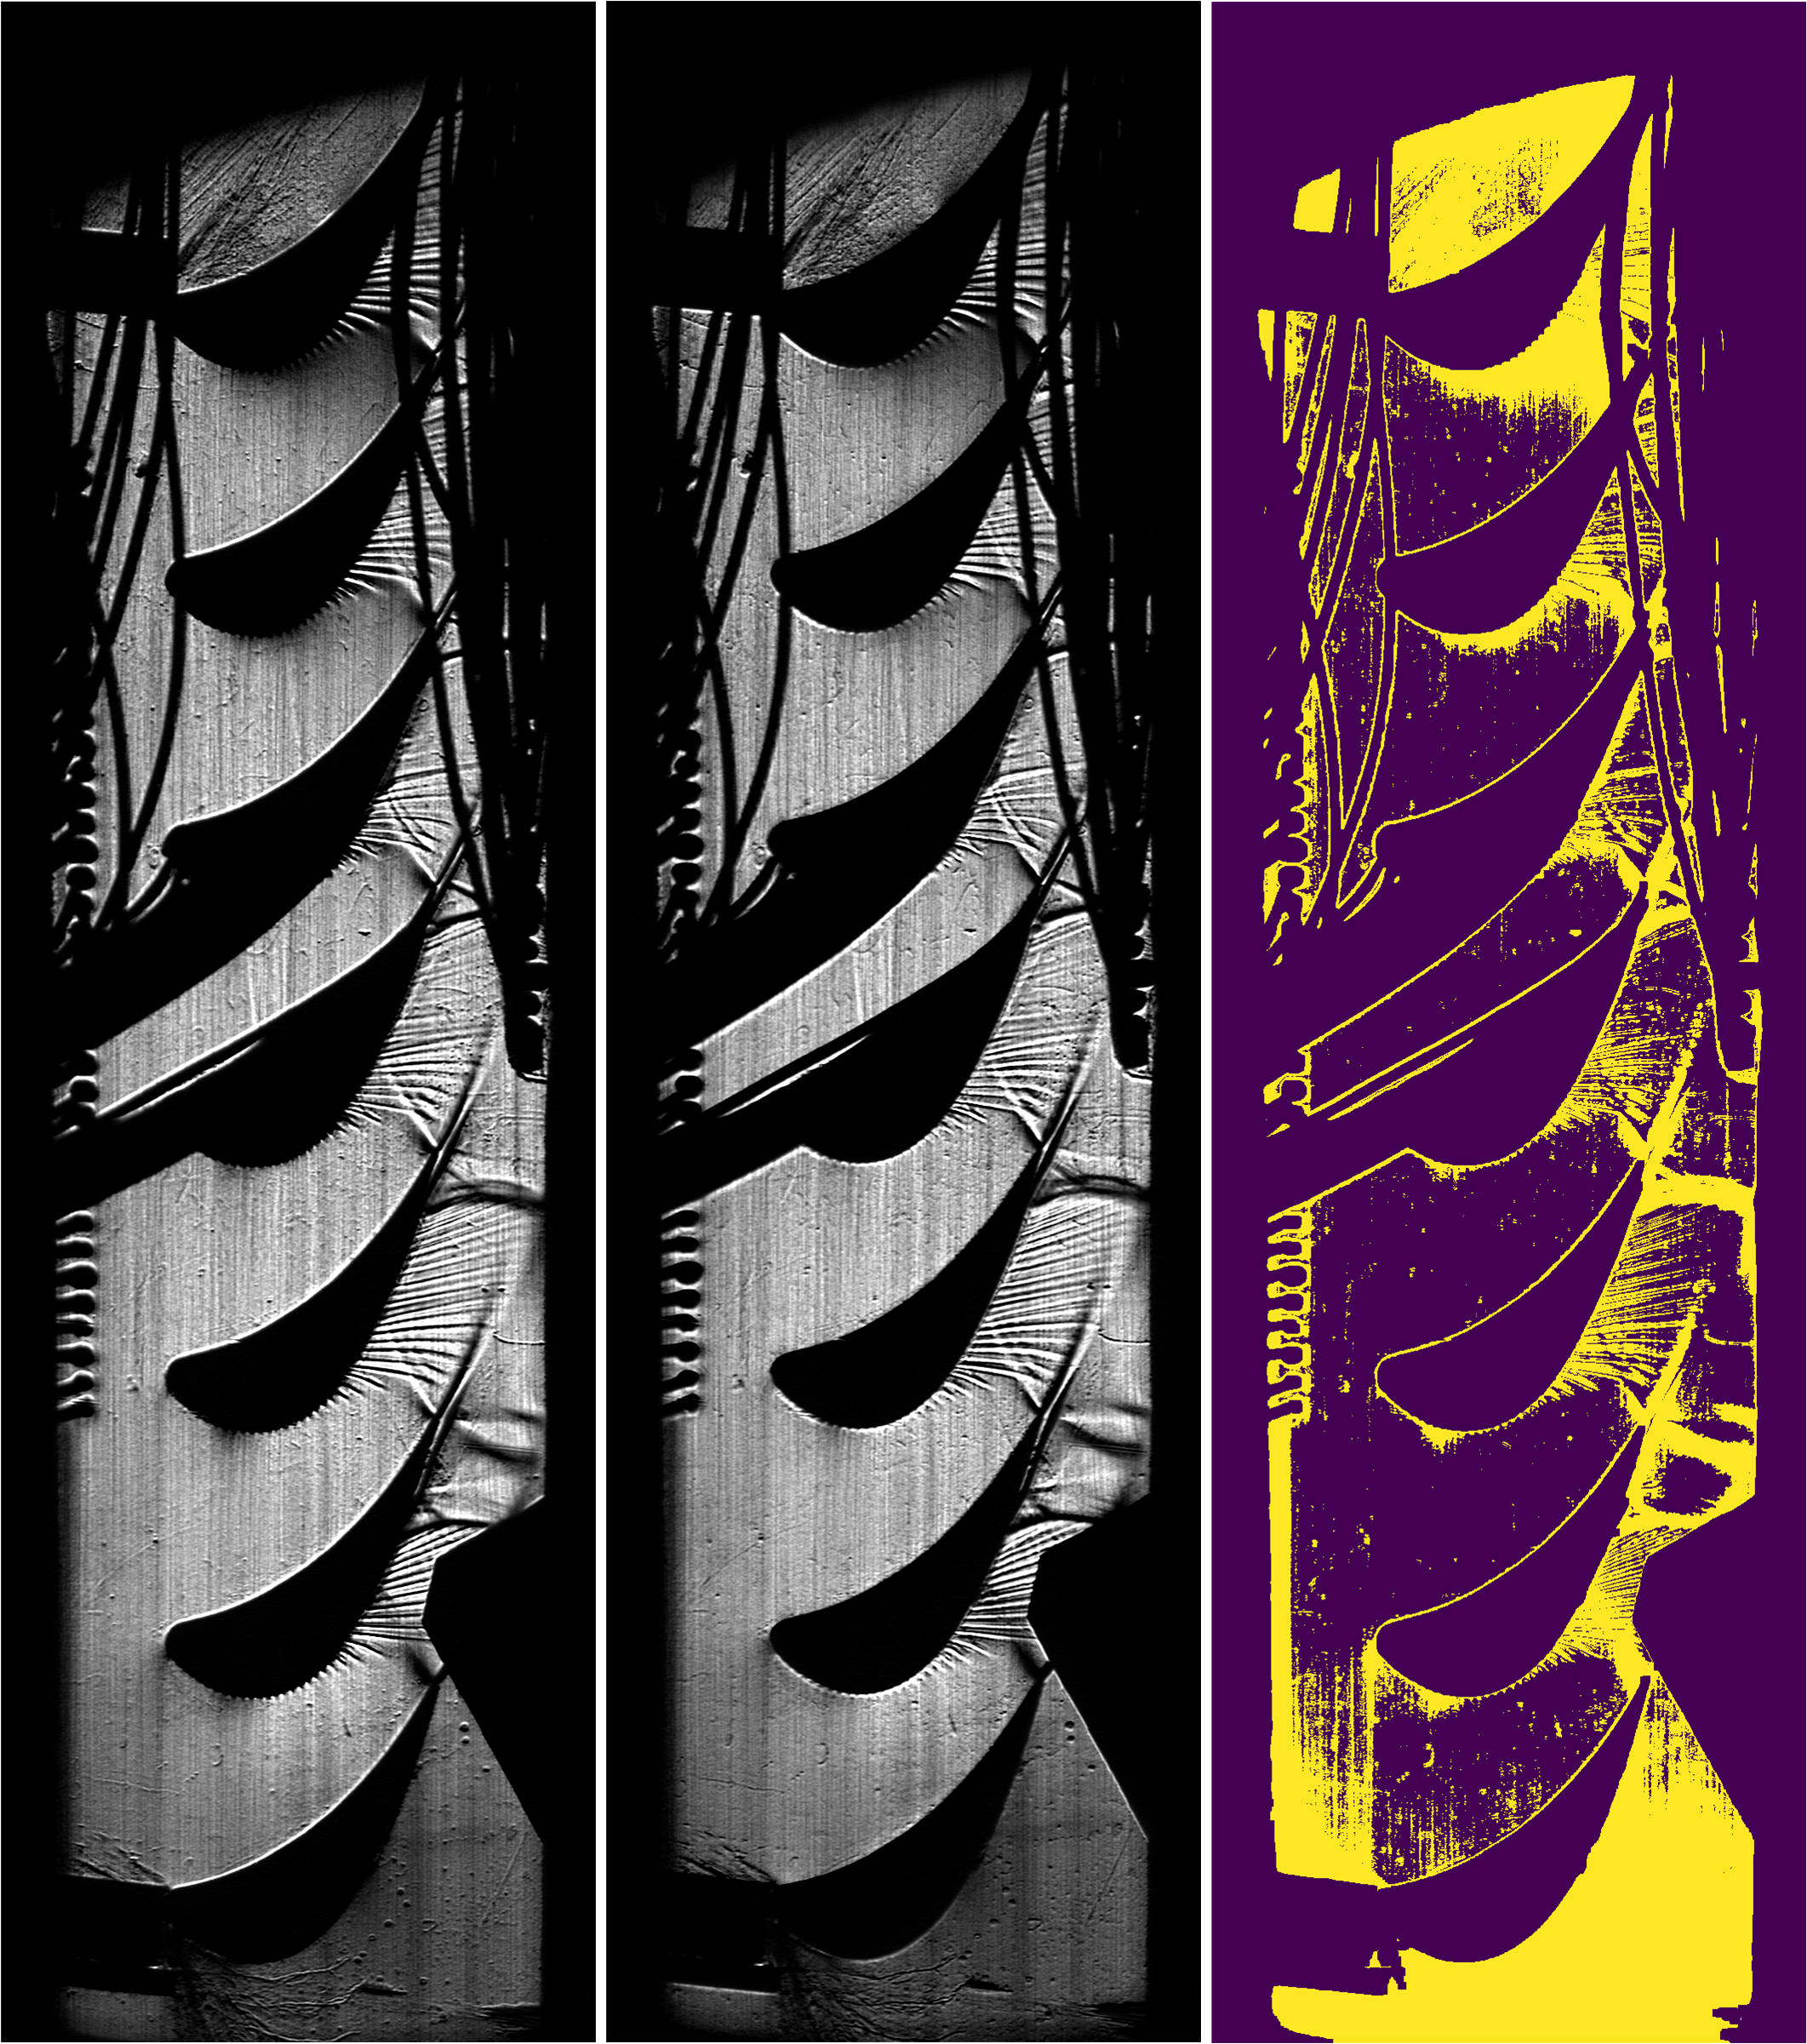
\includegraphics[width=0.75\linewidth]{src/Mf}
	\end{center}
	\caption{ 从左到右依次分别是$I_n$, $I_s$,$M_f$.}
	\label{fig:Mf}	
\end{figure}




\section{Bkg 区域处理}
由于公式\ref{eq:v}, 可得$V_b = V - V_r - V_f$, $V_r, V_f$已知, 即可求得$V_b$. 

综上, 以上三个区域完成分割, 如图\ref{fig:masks}
\begin{figure}[h]
	\begin{center}
		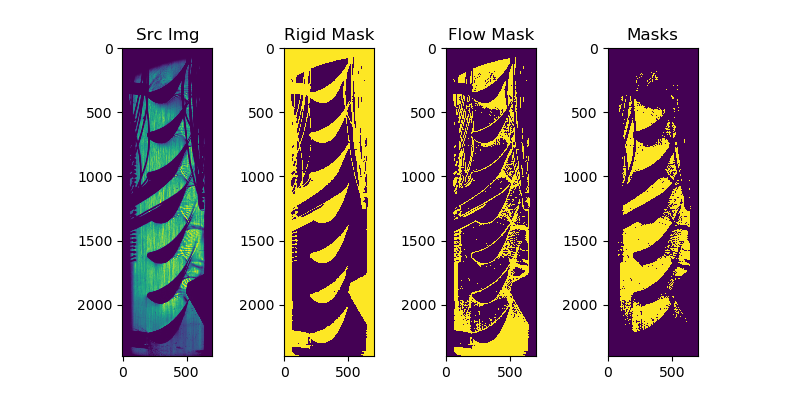
\includegraphics[width=0.95\linewidth]{src/masks}
	\end{center}
	\caption{ \textbf{从左到右依次是$I,~M_r,~M_f,~M_b$}}
	\label{fig:masks}	
\end{figure}



\section{色彩映射(colormap)}

给一张灰度图, 通过色彩映射函数, 可将图像转换成RGB图像或RGBA图像, 这能使得灰度的变化更有层次感,从而更容易分析颜色变化趋势. 这里我们采用"JetMap"函数\footnote{\url{https://www.mathworks.com/help/matlab/ref/colormap.html}}.


JetMap函数为线性分段函数, 公式如下, 作图\ref{fig:jetmap}
\begin{eqnarray}
    \left\{
        \begin{aligned}
            \quad & r = f_r(x)&\\
            \nonumber
            \quad &g = f_g(x)&\\
            \nonumber
            \quad &b = f_b(x)&\\
		\end{aligned}
    \right.
    \quad &\mathcal{F} = (f_r,f_g,f_b)&
    \label{eq:jetmap}
\end{eqnarray}
这里,$\mathcal{F}$为$R^1\Rightarrow R^3$的函数, 为色彩映射函数.
\begin{figure}[h]
	\begin{center}
		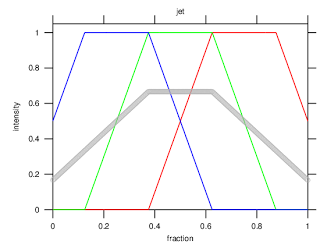
\includegraphics[width=0.75\linewidth]{src/jetmap}
	\end{center}
	\caption{ \textbf{Jetmap色彩映射函数}}
	\label{fig:jetmap}	
\end{figure}


\section{算法流程}
根据原理, 背景处流场密度为整个流场最低, 故将其映射为最低,设为0; 流场区域则根据公式\ref{eq:jetmap}映射, 综上所述,即可得算法\ref{ag:all}:

%\begin{eqnarray}
%    \quad &I_b(p) \rightarrow 0&\\
%    \quad &I_c = I_b + I_f&\\
%    \quad& I^*_c = \mathcal{F}(I_c)&\\
%    \quad&I^*_r(p) = \textbf{r} = [0,0,0]&
%\end{eqnarray}

\begin{algorithm}[h]  
    \caption{Schlieren算法}  
    \label{alg:Framwork}  
    \begin{algorithmic}[1]  
      \Require  
      $I$
      \Ensure  
     $I^*$
     \State $I_b = I\cdot M_b$
     \State $I_r = I\cdot M_r$
     \State $I_f = I\cdot M_f$
     \State $\forall p \in V_b,~~I_b(p) \leftarrow 0$
     \State $I^*_c = \mathcal{F}(I_b + I_f)$
     \State $\forall p \in V_r,~~I^*_r(p) = \textbf{r} = [0,0,0]$
     \State $I^* = I^*_c + I^*_r$
    \end{algorithmic}  
    \label{ag:all}
  \end{algorithm}
其中$I$为原灰度图, $I^*$为最后的渲染图(图.\ref{fig:first_show}右), $I^*_c$为映射后的区域,为RGB图;$r$为自定义的试件和管壁区域的颜色, 这里定义为黑色([0,0,0]); $I^*_r(p)$为Rigid 区域处理后的RGB图.

 



{\small
\bibliographystyle{ieee}
\bibliography{egbib}
}

\newpage
%\include{sup/appendics}

\end{document}
